\documentclass[12pt]{article}
\usepackage[english]{babel}
\usepackage[utf8x]{inputenc}
\usepackage[T1]{fontenc}
\usepackage{lab}
\usepackage{listings}


\Instructors{Alex Mussa, Kevin Johnson}
\LabNumber{2}
\LabTitle{Introductory Electronics}
\LabDate{June 26th, 2019}

\lstset{style=mystyle}

\begin{document}
\MakeLabPrelimTop

\section{Electricity}

The electrical devices used in modern technology are enabled by advancements in the understanding and mathematical representation of the physical phenomena of how various types of materials "conduct" what is known as electricity. Different materials will either permit, in the case of conductors, or restrict, in the case of insulators, electricity to flow through the material. It has become increasingly important to understand electricity as it supplies the power necessary to operate circuit elements which perform tasks such as performing mathematical operations, storing and transmitting information, and producing energy in the form of light and heat. With electricity having such an enormous impact on society through the technologies it enables, developing a theoretical understanding of its physical operation and numerical representation of the phenomenon of electricity has long been researched and established. 

It is important for any electrical and computer engineer to understand various aspects of the nature of electricity in order to develop systems in which its flow can be utilized for important tasks. As such, forming a solid understanding of the impacts of the chemical nature of the materials, the physical nature of the phenomena, and the mathematical representation and manipulation of the phenomena of electricity is critical. Building this intuition enables engineers the tools necessary to create systems that help the human race understand the world we live in better, make robust decisions in critical situations such as cancer diagnosis, perform the communication of information across far distances, allow robots and drones to navigate autonomously, and many more impactful applications on our society. 

\subsection{Conductors, Insulators, and Semi-Conductors}

\begin{figure}[H]
    \centering
    \includegraphics[width=15cm]{photos/prelim/conductorsexamples.png}
    \caption{Conductors, insulators, and semi-conductors real examples.}
\end{figure}

The combinations of the three materials (conductors, insulators, and semi-conductors) form the foundations of understanding electrical technologies, such as those depicted in \textit{Figure 1}. The first image is a pair of wires used in the transmission of power. These wires are composed of an insulator on the exterior to direct and contain the flow of electricity and a conductor to carry it. The second image of an antenna is a large conductor that transmits information in the form of electro-magnetic waves. The red circuit board is a composition of insulator, conductor, and semi-conductor materials and serve to enable electric devices to operate in a compact or confined space. The lightbulbs depicted on the right convert electrical energy to light with the use of insulators such as glass and conductive metals.

The image of the circuit board in \textit{Figure 1} may seem like a complicated object to understand, but at the basis it consists only of insulator, conductor, and semiconductor materials. The configuration of these materials based on how they interact with each other and effect the flow of electricity drive the design and specific placement of these materials on the circuit board. When an engineer has a desire to perform a specific task, this specific topological arrangement becomes the primary tool for successful implementation. 

\subsubsection{Conductors and the flow of current}
\begin{figure}[H]
\begin{subfigure}{.5\textwidth}
  \includegraphics[width=0.95\linewidth]{photos/prelim/Aluminum.png}
  \caption{An atom of Aluminum.}
\end{subfigure}%
\begin{subfigure}{.5\textwidth}
  \centering
  \includegraphics[width=0.88\linewidth]{photos/prelim/metallicbond.png}
  \caption{Metallic Bond formed by Aluminum atoms.}
\end{subfigure}
\caption{An illustration of an atom of aluminum and aluminum bonded to aluminum.}
\end{figure}
Conductors are materials that pass energy in the form of electric charges through the material. Consider the atom of aluminum in \textit{Figure 2 (a)}. When the aluminum atoms combine to form a metallic bond with other atoms of aluminum such as in \textit{Figure 2 (b)}, the 3 valence electrons in the outer orbital of each atom become loosely attracted to its original atom and become free to move from one atom to the next. These free electrons form an "electron sea", where they are free to move with little force. The opposite polarity of charge between two points in the material, caused by the presence of positively charged protons and negatively charged electrons, generates an attracting or repelling force that cause electrons to travel through the material. This potential difference between two points in a material, known as voltage, causes free electrons to attract towards the positive potential and away from the negative as the electrons themselves are negatively charged. This flow of electrons through the material helps define an attribute, known as current, which indicates the amount of charge traveling every second through the material. The amount of charge traveling depends on the resistance of the material and amount of potential difference or voltage between the two points and is dictated by ohm's law which is given below where V is voltage with units volts, I is current with units amperes, and R is resistance with units Ohm ($\Omega$). $$V = IR$$ 

In \textit{Figure 2(b)}, the metallic bond has very little resistance since current can easily flow due to the outer electrons being free to move through the material with ease. As such aluminum is a good conductor of electricity and other commonly used conductor metals include copper, gold, and silver. Since voltage is directly proportional to the product of current and resistance, if a material exhibits a lower resistance value R, then some constant voltage V would supply more current. As R increases, that same voltage produces less current to travel. 

Although metallic bonds exhibit little resistance, no bond is lossless as when the electrons travel through the medium, they collide with each other and the nuclei that form the lattice structure and dissipate energy as heat and electromagnetic radiation such as light. This energy consumption is dependent on  the amount of resistance a material exhibits directly by the relationship below, where P is Power with units watts, V is voltage, and I is current. $$P = VI = I^{2}R = \frac{V^2}{R}$$ 

\subsubsection{Insulators}
An insulator is the complement of a conductor, where very little electrical charges are capable of transmitting through the material typically due to an ionic or covalent bond. In these types of atomic bonds, the valence electrons are not free to move and require a significant amount of energy to free the electrons for mobility. Hence, insulators do not pass electricity. When the outer orbital is completely bonded or has little free electrons, the flow of electricity is restricted. An example of an insulator would be the rubber casing commonly found around an electrical wire as seen in \textit{Figure 1}. Insulators are used around conductors in order to isolate the electricity from flowing to surrounding materials. Some examples of an insulator are rubber, wood, plastic, and glass. 

In many electrical applications, it is necessary to use conductors to effectively transmit the charges from one part of the circuit to another to perform a specific operation. Some real world examples of the combinations of such materials can be seen in \textit{Figure 1}. From the transmission of electricity through power wires to the transmission of information through antennas, conductors, insulators, and semiconductors serve as the foundation that enable the technologies to be useful and feasible in our society.

\subsubsection{Semi-conductors}
\textit{Semiconductors} refer to material compounds that bring some material, such as silicon who naturally has 4 valence electrons, closer to that of a conductor or insulator. When silicon is doped with some other chemical, the outer shell will have a different amount of valence electrons from that of the original Silicon atom. If the amount of valence electrons in the dopant material added to the silcon is 3, only 3 bonds can be made where the fourth is missing an electron. The material is known as a p-type material and that missing electron in the bond is referred to as a "hole". Alternatively, if the dopant material to that of the silicon has 5 valence electrons, all 4 valence electrons of the silicon are used for bonding, and the additional electron from the dopant is free to roam. This material is an n-type material, and that single electron is refered to as just that, an "electron". Using a combination of p-type and n-type materials together form the basis of semiconductor devices and the appropriate configuration of the materials allows the functionality of some important circuit elements, such as Light Emitting Diodes (LEDs) and transistors.

Semiconductor materials form the foundation of several critical technologies such as processors, graphics cards, poweer amplifiers, and storage drives to name a few. The appropriate configuration of the materials allows electricity to be manipulated in a manner that serves a special purpose as designed by the engineer. For now, we will not worry too much about semiconductors but will cover some basic properties such as biasing and turn-on voltage of a diode such as a Light Emitting Diode (LED).

\subsection{Voltage, current, and resistance}
This phenomena of passing an electric charge $(Q)$ such as an electron with units \textit{coulombs} through the conductor material is called \textit{current}. Since the atoms of the conductive material, such as copper, are closely packed together in a solid and only have a free electron after the metallic bond, electrons are free to move from one atom to the next. That is, as charge is passed through a material from atom to atom overtime, current is an important quantity to know, having units of \textit{Amperes (A)} which are expressed as $\frac{coulombs}{second}$. 

It is such that if a material has a higher \textit{conductivity}, then more \textit{current} can pass through it due to the material exhibiting a lower \textit{resistance}. Resistance $R$ is defined as the inverse of conductivity $G$ such that $R = \frac{1}{G}$. Resistance has the units of Ohms ($\Omega$), where conductance has the units of Siemens (S). The value of conductivity is material dependent; Each material has a different value of conductivity and thus a different value of resistivity. These values are important for understanding how much power will be expected to be lost when choosing the conductor.

 Voltage is defined as the difference in \textit{electric potential} between two points in space. Here, electric potential refers to the amount of work needed to move a unit of charge (Q) from one point to another. Without worrying too much about the literal definition of voltage, its simpler to observe the relationship between voltage, current, and resistance through what is known as \textbf{Ohm's Law} and was stated previously as $V = IR$.
Think of a fixed resistance device, known as a resistor. If the resistance doesn't change, lets say $R = 1 \Omega$, then the amount of current that flow through the resistor is directly proportional to the voltage that is applied. In this respect, if 5 Volts of potential difference is applied across the resistor, then 5 Amperes of current will flow from one end to the other. The voltage is the force that drives the charge to flow through the resistive medium. 

\subsection{Voltage variations over time: AC vs DC}

As time elapses, the value of the current can change or remain the same, depending on the source from which the power is being supplied. Two types of time-variations for voltage and current are \textit{Alternating} and \textit{Direct}. Alternating Current (AC) has values of current that vary periodically with time, such as the sine wave  shown in \textit{Figure 3(a)}.  Note that with a fixed resistance, the alternating nature of the voltage produces the alternating nature of the current and vis-a-versa. In this manner, the current changes travel direction and magnitude continuously, causing the electrons to osillate back an forth. This oscillation causes vibrations of the electrons not found in DC.

\begin{figure}[h]
\begin{subfigure}{.5\textwidth}
  \includegraphics[width=1\linewidth]{photos/prelim/AC.png}
  \caption{AC Voltage Waveform}
\end{subfigure}%
\begin{subfigure}{.5\textwidth}
  \centering
  \includegraphics[width=1\linewidth]{photos/prelim/DC.png}
  \caption{DC Voltage}
\end{subfigure}
\caption{An AC voltage waveform and a DC voltage plotted against time.}
\end{figure}

Direct Current (DC) has a constant value of current that does not change at any instant of time. Batteries typically store and produce a DC, where the electricity that comes from the outlet found in residential or commercial locations are AC. As such, in order to charge a battery, the current must be converted from an alternating to direct current.

AC and DC voltages have different parameters that specify their composition. DC is more simple, as only one value is utilized to specify it. This value is Amplitude, depict by the A in \textit{Figure 3 (b)}. Alternatively, AC voltage can take many waveforms, such as the sinusoid waveform seen in \textit{Figure 3 (a)}. Each waveform has different parameters that specify it, but most share some of the common ones found in the sinusoid due to their periodic natures. Some parameters to note in the sinusoidal waveform are the amplitude of a single peaks voltage $V_p = A$, peak-to-peak voltage $V_{pp} = 2A$, and the frequency. The frequency of the waveform is dependent on how much time elapses before the waveform starts to repeat itself, known as the period. Observing the waveform in \textit{figure 3(a)}, notice that the wave from time $t=0 \longrightarrow t=T$ and from $t=T \longrightarrow t=2T$ are identical. In this sense, the signal is periodic with time duration T. That is, every T seconds, the waveform or signal repeats itself. From this period value of T, the frequency of the signal can be computed as $f = \frac{1}{T} Hz$. Intuitively, this value tells you how many cycles of the periodic waveform occur every second. For example, if one cycle of the waveform occurs every half of a second, then the signal is said to oscillate at a frequency of 2 Hz, as for every 1 second there are 2 cycles of the signal that occur.

\subsection{Example of Circuits: The Arduino}

The arduino microcontroller will be utilized in this class as the brain of the controls for the self-balancing robot. The Printed Circuit Board (PCB) that the arduino microcontroller is housed on as well as the accompanying circuit elements is entirely composed of insulators, conductors, and semiconductors that are pieced together to serve the purpose of controlling the robot. A thorough description of where these materials are found and why they are used for the PCB seen in \textit{Figure 4} is as follows.

\begin{figure}[H]
    \centering
    \includegraphics[width=15cm]{photos/prelim/arduinolabeled.png}
    \caption{The arduino nano microcontroller.}
\end{figure}

\begin{enumerate}
    \item The PCB's main body material is an insulator, of which is typically fiberglass (glass threads bound in resin).
    \item The light blue lines on the PCB are where traces (solid paths) of copper conductor are visible under the insulating blue mask. The dark blue areas between the traces have no copper, and isolate the nodes of the circuit, preventing them from interacting with each other.
    \item When the copper trace arrives at a circuit element such as those in 4 and 5, a small amount of solder (a mix of tin and other metals like lead or silver) connects the trace to the circuit elements contacts. 
    \item The circuit elements on the PCB are important in the operation of the device. These circuit element include resistors, diodes, LEDs, push buttons, the microcontroller itself, and other integrated circuits (IC's).
    \item The connection terminals such as the pin headers and USB port are composed of both insulating and conductive materials. These allow the circuit on the PCB to interface with external electronics such as computers for programming the microcontroller and sensors for interaction with the physical world.
\end{enumerate}

With knowledge of these materials, engineers are able to design the layout of such a PCB in a manner as described above to route AC and DC signals to different components which perform different tasks that enable the system to control a robot, for example. Engineers are also able to manipulate semiconductor materials to help perform mathematical computation on voltages on a very small scale which can be utilized for very important tasks. In order for these tasks to be successfully completed, the amount of electricity required to operate the device is an important aspect of a device to study. To quantify this amount, a complete circuit schematic of the system must be developed and analyzed. The next section discusses circuit elements, how to interpret a circuit schematic, and how to perform basic calculations on it. 

\section{Circuit Elements}
\subsection{Schematics of Basic Circuit Elements}

A typical circuit is composed of a power source such as a battery or power supply, some conductor such as wire, and some circuit element as a load such as a resistor. A simple circuit schematic can be seen below.

\begin{figure}[h]
\begin{subfigure}{.5\textwidth}
  \centering
  \includegraphics[width=0.5\linewidth]{photos/prelim/circuitschmeaticlegend.PNG}
\end{subfigure}%
\begin{subfigure}{.5\textwidth}
  \centering
  \includegraphics[width=0.8\linewidth]{photos/prelim/circuitschmeatic.png}
\end{subfigure}
\caption{A simple circuit schematic and its symbols.}
\end{figure}

In \textit{Figure 5}, the lines connecting the positive terminal of the battery to the resistor and connecting the negative battery terminal, the resistor, and the ground symbol, are wires. Notice the polarity of the battery. It is important to keep this in mind when analyzing the circuit, because the direction of the current depends on it. Electrons are emitted or repelled from the negative terminal and attracted toward the positive terminal of the battery. Although this is the case, the direction of current when analyzing circuits is opposite the direction of the flow of electrons, as depicted in \textit{Figure 2(b)}.

The ground element in this circuit serves as the reference for "0 volts". If the battery is rated at 5 volts of potential difference, that means that the potential difference the battery supplies is 5 volts between its two terminals terminal. When analyzing circuits, it is useful to define one node as 0 V, and often a sensible node is designated by the designed using the ground symbol.  The use of the word ground here stems from the fact that the earth itself is often defined as 0 V, and in many cases (such as with household power sockets) metal rods are literally placed into the ground to provide a common voltage reference for everything plugged into the wall. The ground symbol in schematics, however, does not necessarily need to lead to the ground of the earth and can just be a point of reference for voltage potential and a return path for the electric current.

\subsection{Batteries}
One area you may have heard of voltage being used in is the specifications of a battery. The various batteries you may have heard of, such as AA, AAA, C, D, etc., are classified on several specifications including nominal output voltage and storage capacity. The storage capacity here is the amount of charge the battery can contain at max. Recall from earlier the quantity of power (P) as the product between voltage and current. That is: $P = VI$ Note that power has the units of Watts (W).

Batteries are limited in their capacity, which means that a battery can only store so much charge and can become depleted. The battery's capacity is typically measured in Amp-hours, dictating the amount of time in hours a current draw of however many amps can be pulled from the battery before the battery has been depleted. Note that the battery has a fixed voltage, and thus the life of the battery depends completely upon the current draw of the \textit{load} that is applied to it.

For example, if a battery has a nominal voltage of 5V and a capacity of 2 Ah, how long could the battery supply power to a $10\Omega$ load? From the battery, $I = \frac{V}{R} = \frac{5V}{10\Omega} = 0.5 A$. As such, it will take $t = \frac{2Ah}{0.5A} = 4h$ or 4 hours. Note this calculation is approximate in that the actual output voltage varies with time and does not remain at 5V.

An intuitive example of this is your cell phone. The load is everything that uses power in the cell phone itself (screen, processor, applications, etc.). Take the backlight into consideration. If you dim your backlight on the screen of your phone, you are reducing the amount of current supplied to the LEDs. This in turn causes less current to be drawn from the battery, and increases the duration for which the battery can be used before depletion.  

\subsection{Resistors}

Resistors in circuit are typically composed of conductive legs on each side that lead into a resistive material. Inside is a thin carbon, metal, or metal oxide somewhat-conductive material that inhibits the flow of electricity. An example of a through-hole resistor can be seen below.  

\begin{figure}[H]
    \centering
    \includegraphics[width=15cm]{photos/prelim/resistors.png}
    \caption{Through-hole resistors used in circuits.}
\end{figure}

When a potential difference is applied at the wires depicted in the \textit{Figure 6}, current will flow through the resistor body based on the amount of resistance and voltage applied. The color code located on the resistors body by the colored lines represents the amount of resistance the material within the resistor body introduces. It is not expected for you to be able to calculate the resistance from these colors, but just to know that they signify the resistance value. 

\subsection{Basic Circuit Analysis on a Resistor}

To show how various conditions of potential differences applied across a resistor effect the direction and flow of current, consider the circuit in \textit{Figure 7}. In this circuit schematic, we have a resistor with two different voltages, $V_1$ and $V_2$, applied to left and right hand sides of the resistor respectively. Note that the batteries are connected to the same ground, so $V_1$ and $V_2$ reference their voltage from the same 0 V node. 

\begin{figure}[h]
    \centering
    \includegraphics[width=8cm]{photos/prelim/circuitschmeatic2.PNG}
    \caption{An example of different voltage conditions on each side of a resistor.}
\end{figure}

For the case when $V_1 = V_2$, no current will flow through the resistor, because when the same voltage is applied to both sides of the resistor, there is no voltage drop across the resistor. Without a voltage drop from one side to the other, the value of V in the equation for ohm's law is 0 and since the resistor is a finite non-zero value, the current must also be zero.

For the case when $V_1 > V_2$, current will flow from left to right through the resistor, or from the $V_1$ battery to the $V_2$ battery. The amount of current flowing through the resistor is dependent upon the difference between the voltages $V_1$ and $V_2$. As an example, consider $V_1 = 5V$, $V_2 = 2V$, and $R = 3k\Omega$ where $3k\Omega$ refers to 3 kilohms which is $3000\Omega$. Here, the voltage drop across the resistor is $V_1 - V_2 = 5V - 2V = 3V$ and so the amount of current flowing through the resistor is $I = \frac{V}{R} = \frac{3V}{3000\Omega} = 0.001 A = 1 mA$ where 1 mA means 1 miliamp. 

Similarly, for the case when $V_1 < V_2$, current flows from right to left or from the $V_2$ battery to the $V_1$ battery. Note that, in this circuit, the current flowing through all of the wires is equal to 1mA. The wire connecting battery $V_1$ to the resistor is at a voltage of $+V_1$ and the wire connecting $V_2$ to the resistor has a voltage of $+V_2$.  Again, the wire connected to ground is at, by definition, $0V$.

\subsection{Basic Circuit Analysis on a Series and Parallel Combination of Resistors}
In many circuit applications, multiple circuit elements will be used in combination with one another, forming connection configurations known as series and parallel. In these types of situations it is important to know the parameters such as voltage and current that will occur within any given circuit element at some point in time while it is operating. The underlying cause of current to travel through the circuit as it does is dictated primarily by ohms law and some knowledge of the materials configuration.

\begin{figure}[H]
\begin{subfigure}{.5\textwidth}
    \centering
    \includegraphics[width=0.7\linewidth]{photos/lab/series.PNG}
    \caption{Series resistors.}
\end{subfigure}%
\begin{subfigure}{.5\textwidth}
  \centering
  \includegraphics[width=0.8\linewidth]{photos/lab/parallel.PNG}
  \caption{Parallel resistors.}
\end{subfigure}
\caption{Examples of series and parallel resistors in a circuit schematic.}
\end{figure}

For a series configuration, such as the one seen in the schematic in \textit{Figure 8(a)}, the two resistors are connected "in series" meaning the current must flow through the series of the first into the second. What this means is there is only one path of electrically conductive material for the electricity to flow through, and thus all of the current that will be supplied from the voltage source will flow through both resistors equally. With this notion, the currents labeled in the figure for resistors R1 and R2 are equal, such that $I_{1} = I_{2} = I_{V1}$. It is also important to notice that the total voltage drop between both resistors can only be the value of V1. So, this mean that the sum of the voltage drops across the resistors must be equal to V1, i.e. $V_{1} = V_{R1} + V_{R2}$ Considering that R1 and R2 are fixed resistances, you can replace the voltage drops with the current and resistances product, as dictated by ohm's law such that $V_{1} = I_{1}*R_{1} + I_{2}*R_{2} = I_{V1}*(R_{1} + R_{2})$. As V1 is fixed and know,  it can be viewed that the equivalent resistance of the circuit seen by the voltage source can be computed as $R_{series} = \frac{V_{1}}{I_{V1}} = (R_{1} + R_{2})$. This resistance is know as the series resistance and can be applied for any N resistors in series, such that $R_{series} = \sum^{N}_{i=1} R_{i}$.

For a parallel configuration as seen in \textit{Figure 8(b)}, the current has two paths to take and as such the current through each resistor may not be the same. The only time they will be the same is if each path has the same amount of resistance. In other situation, the current will travel more through the less resistance, as dictated by the facto both resistors are supplied with the same voltage. Ohms law shows that if $V_{R3} = V_{R4} = V_{2}$, then the amount of current being supplied by the power supply $I_{V2}$ can be computed as the sum of the current traveling through the two resistive loads in the circuit, $I_{V2} = I_{3} + I_{4}$. To solve for the equivalent resistance seen by the power supply, the previous equation can use ohms law to be rewritten as $I_{V2} = \frac{V_{R3}}{R_{3}} + \frac{V_{R4}}{R_{4}} = \frac{V_{2}}{R_{3}} + \frac{V_{2}}{R_{4}} = V_{2} * (\frac{1}{R_{3}}+\frac{1}{R_{4}})$, so $R_{parallel} = \frac{V_{2}}{I_{V2}} = \frac{1}{(\frac{1}{R_{3}}+\frac{1}{R_{4}})} = \frac{R_{3}*R_{4}}{R_{3}+R_{4}} $. This can be generalized for N resistors
such that $R_{parallel} = \frac{\prod^{N}_{i=1} R_{i}}{\sum^{N}_{i=1} R_{i}}$.

\section{Building Physical Circuits}

When building a physical circuit, various components are combined together in a specific way to allow the flow of electricity in the desired manner. In the lab, you will use a device called a "breadboard" or "protoboard" to connect all of these pieces together. These breadboards are convenient for prototyping and testing circuits. Alternatively, when a final design is completed, it is desirable to print the circuit onto a PCB. However, in the lab we will be working with experimenting and prototyping, so we will utilize a breadboard for our circuits. 

\subsection{Breadboard}

\begin{figure}[h]
    \centering
    \includegraphics[width=15cm]{photos/prelim/breadboard_labeled.png}
    \caption{An image of a standard breadboard.}
\end{figure}

When building a physical circuit, various components are combined together in a specific way to allow the flow of electricity in the desired manner. In the lab, you will use a device called a "breadboard" to connect all of these pieces together, as seen in \textit{Figure 9} above. The breadboard contains holes where wires and circuit elements can be plugged into. However, knowledge of the topological layout of the breadboard is necessary to successfully build a circuit on one.

The top and bottom of the breadboard have two "rails", which are often used to carry power (i.e. the supply voltage), since that is often needed at many places in the circuit. The holes contained within each of the boxes labeled "power rail" in the figure are all internally connected. When dealing with power on the breadboard, it is always important to BE CAREFUL to not connect ground to power with a wire as a wire has extremely low resistance, so if unimpeded, a large amount of current will flow and cause the wire to melt. These power rails will typically hold your positive voltage supply (from a battery or power supply), negative voltage supply, or ground connection. For the breadboards we will use in lab, this is not necessary as they are internally connected.

In the center of the breadboard are several "node" connections. Each node has 5 connection points which are all connected together. Notice the numbers and letters on the breadboard. It is such that for the "column" number 1 that "row" letters A through E are all internally connected and also letters F through J are also internally connected. Notice that at the blue star in the figure there is a large space between the two nodes in column 1. This spacing is here for integrated circuits with a DIP packaging, such as the DIP-8 package shown in \textit{Figure 10} below. The notch on the left side of the packaging indicates how to identify the numbering of the pins, with the help of the manufactures specification sheet that accompanies the IC. 

\begin{figure}[H]
    \centering
    \includegraphics[width=12cm]{photos/prelim/DIP8.png}
    \caption{A standard DIP-8 packaged IC.}
\end{figure}

The above IC is being inserted with its pin 1 in column 35, row F, so all of the breadboard holes in column 35 rows G-J are connected to that pin. Pin 8 of the IC is being inserted across the gap, at 35E, which is not connected to 35F. In this way, all eight pins of the IC package are isolated from each other, and have four available connections on the breadboard for interfacing with.

Note that any node can be connected with wire to another node to expand the number of connections a single node contains. In essence, the nodes are just a connection of conductor (metal) underneath the insulator (plastic) that connect the points of the node together. As such, they can also be connected to each other with more conductors, such as wires.

\subsection{DC Power Supplies}

Previously, the voltages in the circuit schematics were being supplied by batteries. In the lab, DC power supplies are much more effective to use as they can easily have their voltage level varied with the turn of a knob and do not become depleted of charge. 

\begin{figure}[H]
\begin{subfigure}{.5\textwidth}
    \centering
    \includegraphics[width=1\linewidth]{photos/prelim/powersupply.jpg}
    \caption{A bench DC power supply.}
\end{subfigure}%
\begin{subfigure}{.5\textwidth}
  \centering
  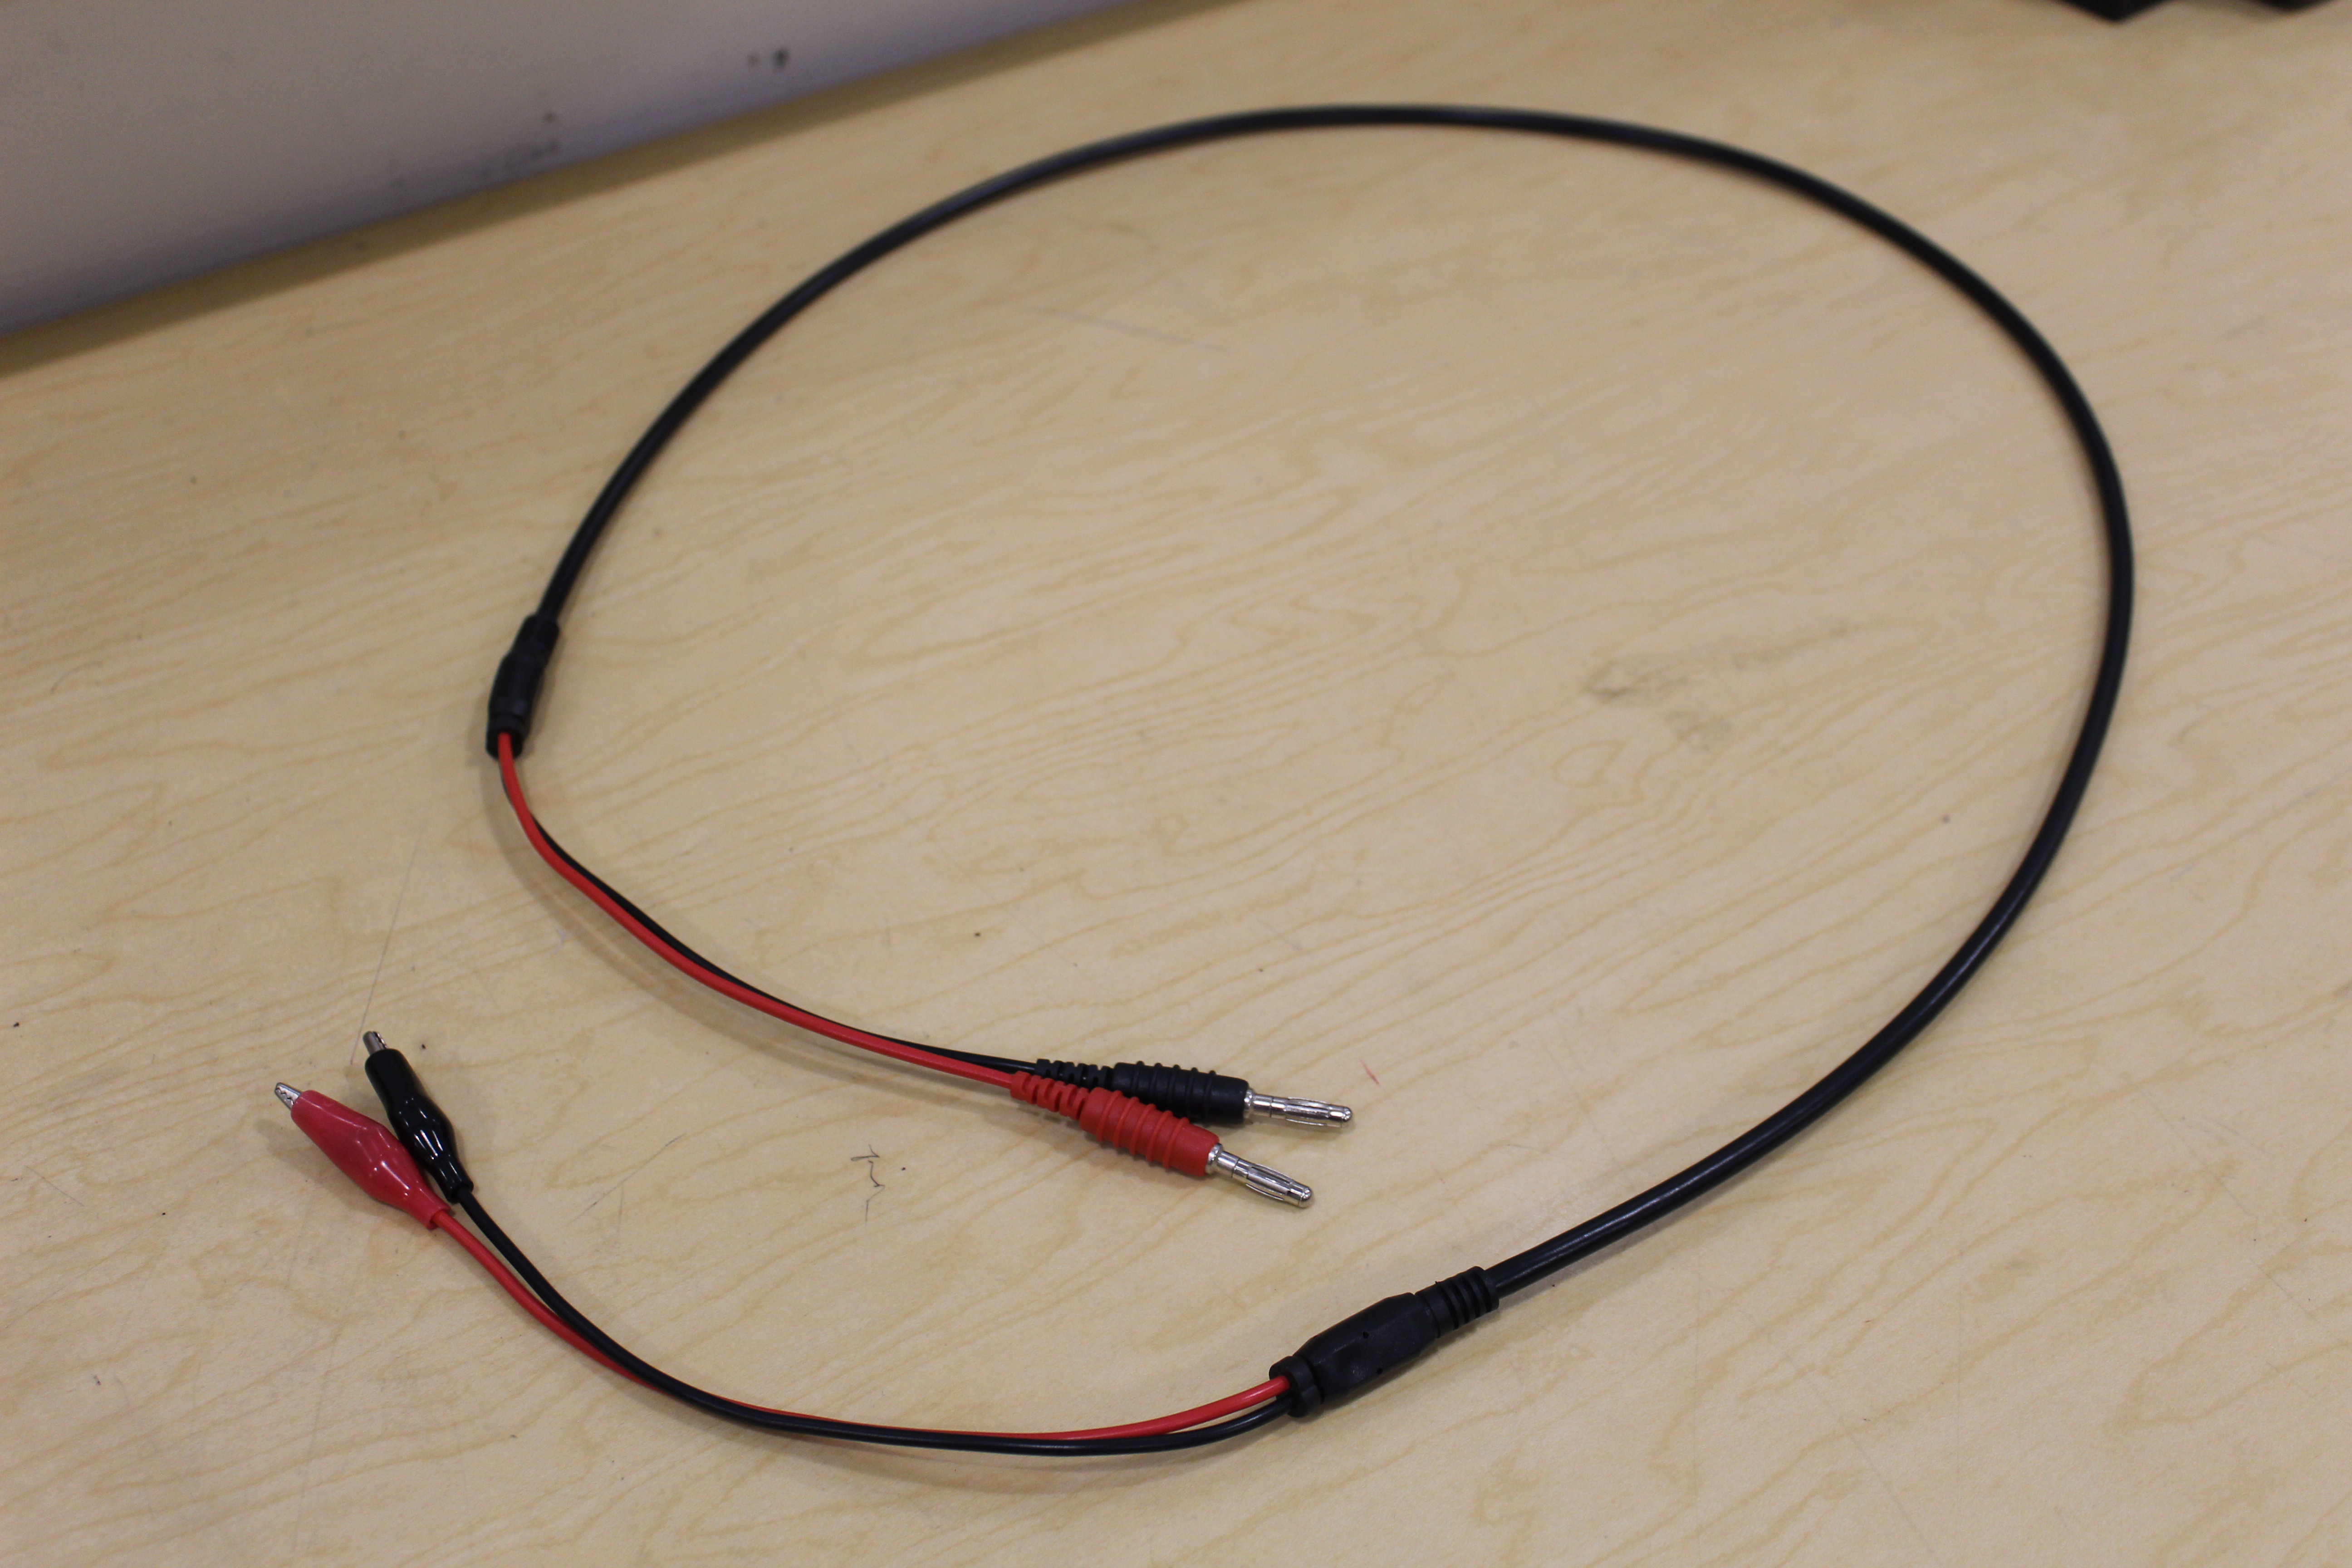
\includegraphics[width=0.8\linewidth]{photos/prelim/bananagator.JPG}
  \caption{A Banana to Alligator Clip cable for the DC power supply.}
\end{subfigure}
\caption{Examples of a waveform generator and a cable used with the generator.}
\end{figure}

The power supply depicted in \textit{Figure 11(a)} has three output voltages. Each is set with the adjustment knob located in the upper right. The tracking ratio here varies the $-20V$ terminal, where if it is set to fixed, the $-20V$ terminal will take the same voltage as the $+20V$ terminal, but negated. As the tracking ratio changes from fixed, the $-20V$ terminal will differ from that of the $+20V$ terminal. Each voltage output has an output terminal that supplies the desired voltage in comparison to the COM output terminal. As such, the voltage output terminal could be seen as the positive terminal of the battery and the COM terminal the negative. In this sense, the positive and negative terminals of the batteries depicted in the previous circuit schematic in \textit{Figure 4} can simply be replaced with the power supply leads. For example, the red terminal of $+6V$ of the power supply would connect to the left side of the resistor in the circuit of \textit{Figure 4} and the red COM terminal is considered the ground or reference point. The $V_2$ could be supplied by the $+20V$ terminal, which would then connect to the right side of the resistor.

In order to supply the voltage from the DC power supply to a circuit on a breadboard, the banana to alligator cable shown in \textit{Figure 11(b)} can be utilized. The male banana connector on the one end of the cable fit directly into the female banana connector of the power supply. The black connector would typically serve as the reference or ground terminal and connect to the COM port on the power supply where the red would connect to the desired voltage output terminal. The alligator clips on the other end of the cable are used to clip onto one end of a wire which can be inserted into the breadboard, such as into the power rails at the top, to utilize for powering circuits.

\subsection{Waveform Generators}

In some circuit elements, AC waveforms are necessary to complete a specific task. In order to generate an AC waveform for prototyping in the lab, a special piece of equipment known as a waveform generator is utilized. The waveform generator found in the lab can be seen below in \textit{Figure 12(a)}.

\begin{figure}[H]
\begin{subfigure}{.5\textwidth}
    \centering
    \includegraphics[width=1\linewidth]{photos/prelim/wavegen.jpg}
    \caption{A waveform generator to generate AC signals.}
\end{subfigure}%
\begin{subfigure}{.5\textwidth}
  \centering
  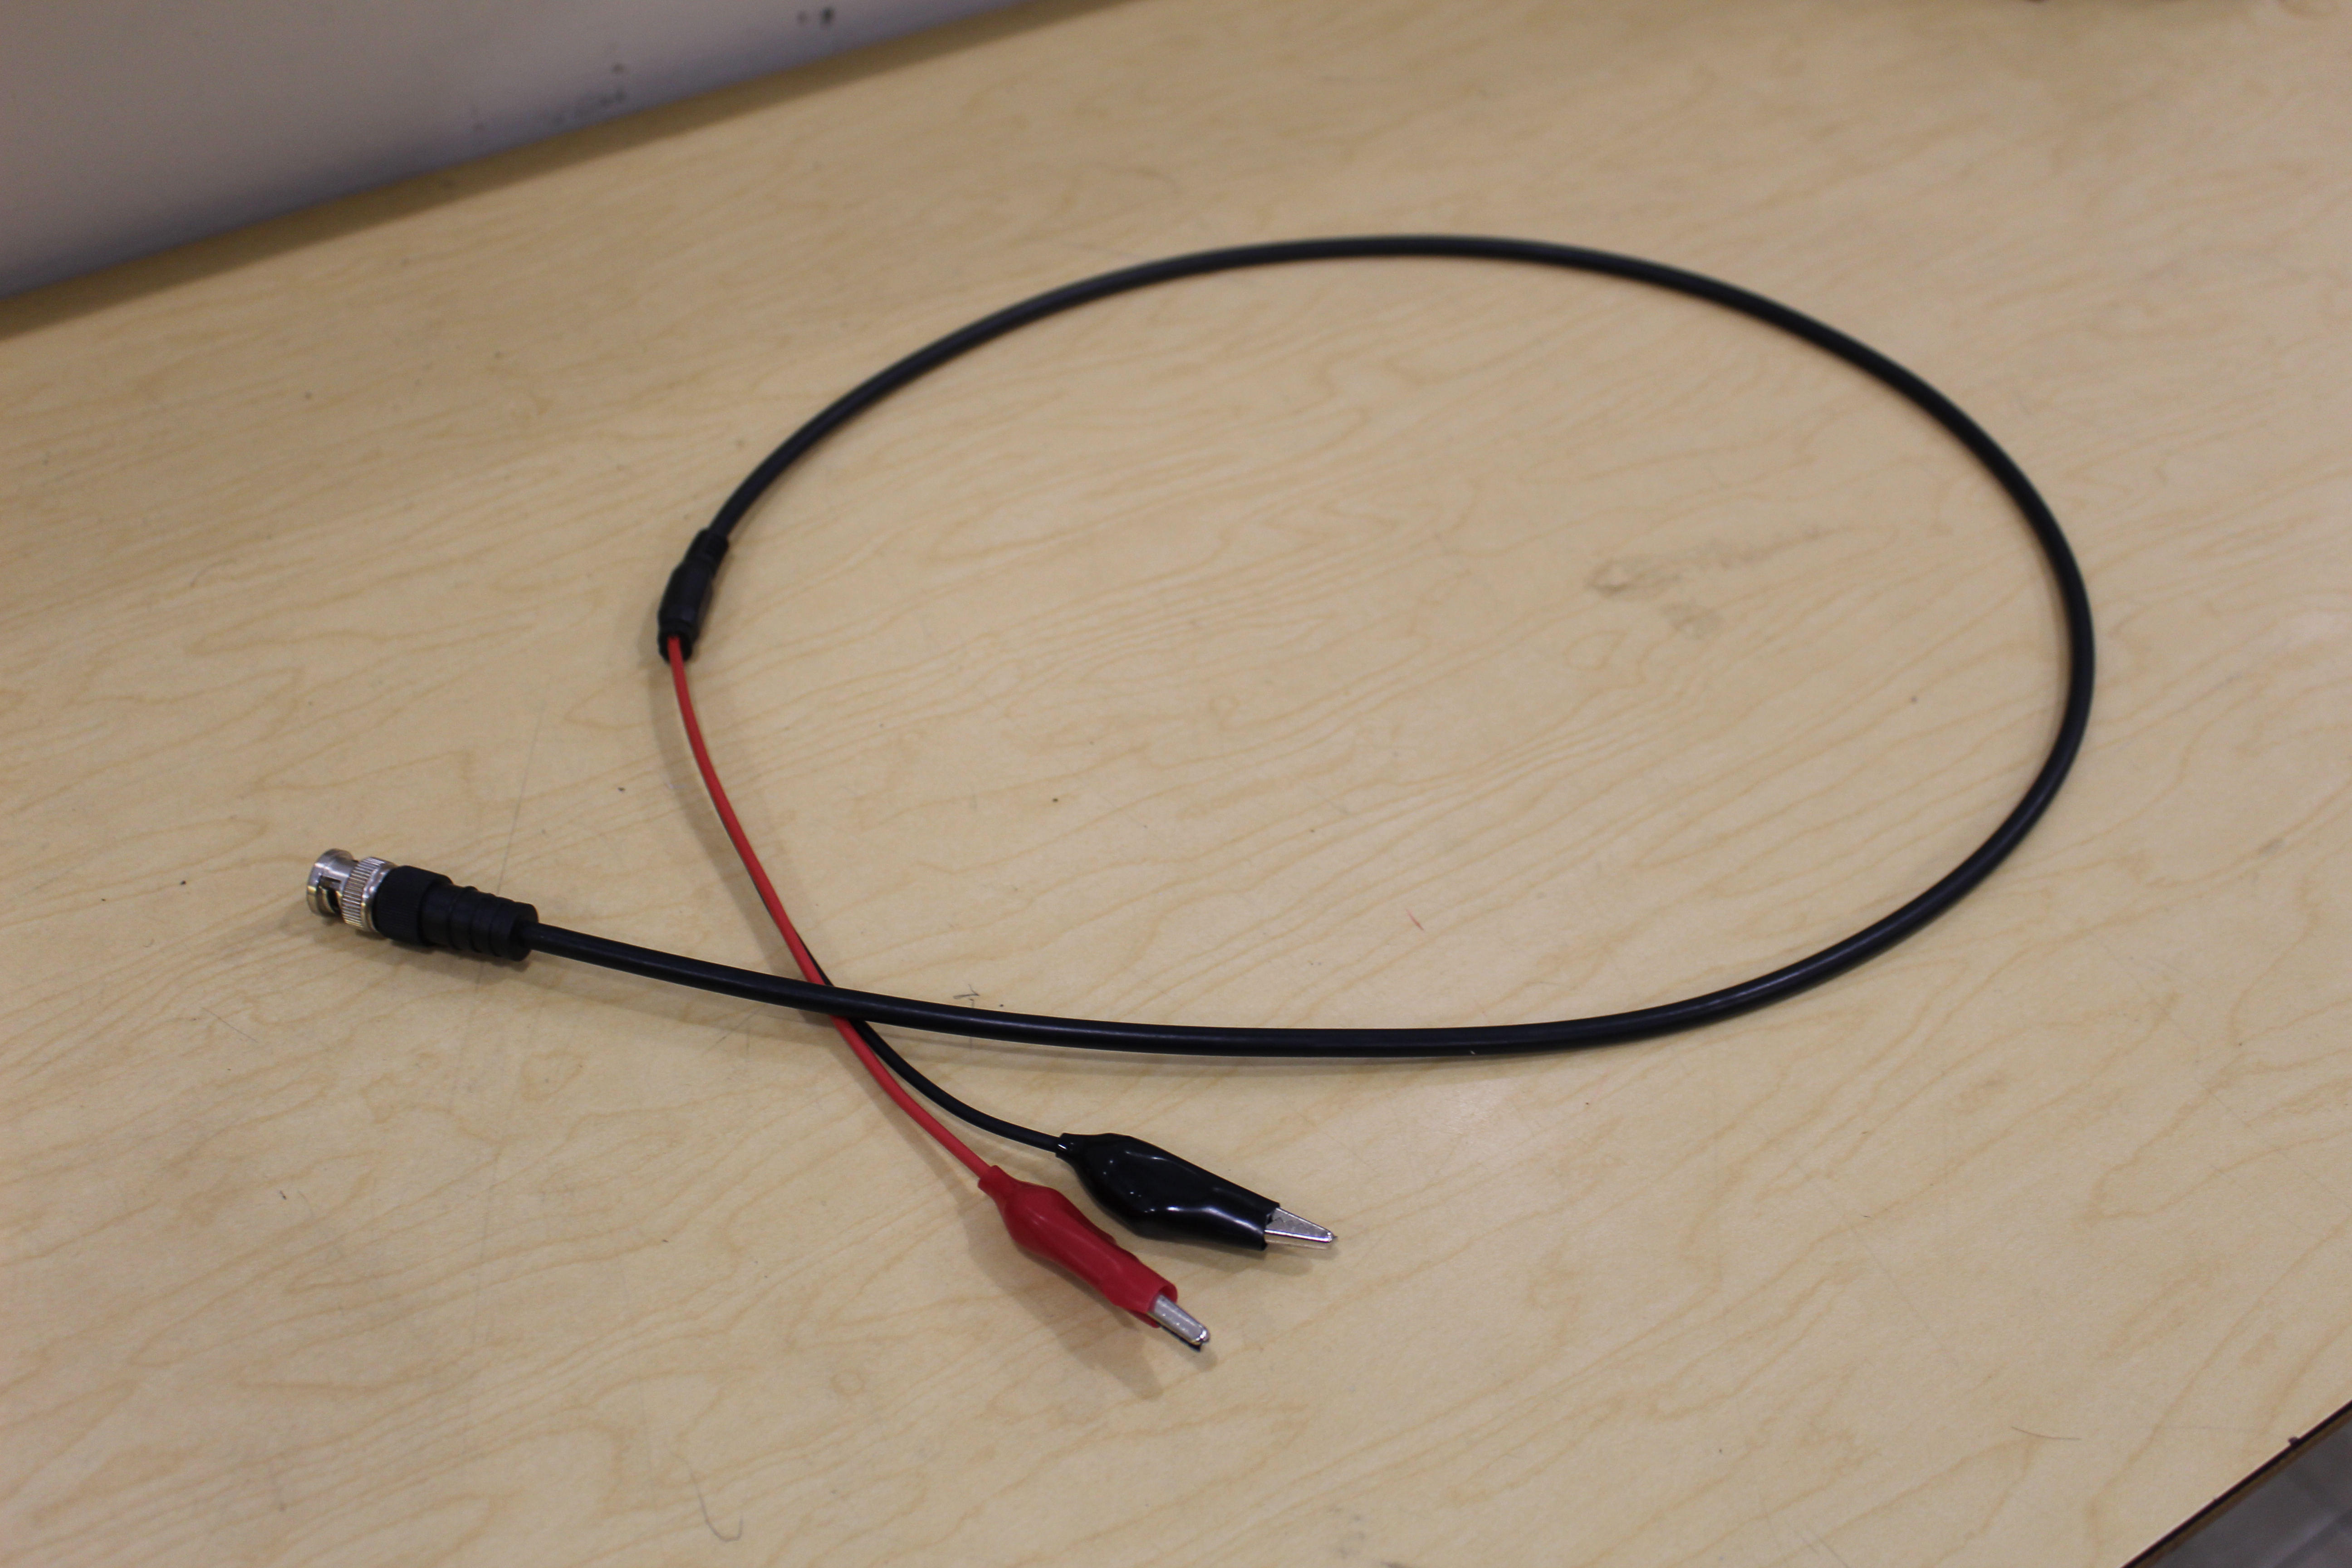
\includegraphics[width=1\linewidth]{photos/prelim/bncgator.JPG}
  \caption{A BNC to Alligator Clip cable for the waveform generator.}
\end{subfigure}
\caption{Examples of a waveform generator and a cable used with the generator.}
\end{figure}

This device has a digital display which is utilized to input the necessary parameters of the waveform, such as the frequency and amplitude as described in the previous section on AC voltages. Other types of waveform other than the sinusoid, such as the square wave, triangular wave, and pulse wave, are available for generation. Each waveform can be used for different circuit elements which require alternating voltage values as opposed to discrete ones. However, the waveform generator can also produce a DC voltage.

The waveform is output at the metal connector seen in \textit{Figure 12(a)}. This connector is called a BNC type connector and is one of many different types of test cable connectors you will find in the lab. As such, the male BNC connector at the waveform generators output can connect with the female BNC connector on the cable shown in \textit{Figure 12(b)}. On the other end of the cable is another type of connector, called alligator clips. These connectors are convenient for clipping onto wires that are then inserted into the breadboard to complete a circuit. The red alligator clip serves as the voltage output, where its supplied voltage is in reference to the black alligator clip.

\subsection{Wires}

In order to connect the power to the breadboard as well as connect circuit elements together, a conductor is needed. Electrical wires contain a conductive metal in the center, as well as an insulator material sleeve over the wire to isolate the transmission of the electricity. For convenience, the wires provided for lab are jumper wires and have connector tips on them as seen in \textit{Figure 13}. 

\begin{figure}[H]
    \centering
    \includegraphics[width=10cm]{photos/prelim/wire.png}
    \caption{Jumper Wires}
\end{figure}

The male end can be used to plug directly into the female slots of the nodes of the breadboard, as well as into the female connector. The wire kit contains male-to-male, male-to-female, and female-to-female wires for use in prototyping. The female connector are convenient for connecting to header pins on devices such as the arduino and can be used to connect with a male connector or exposed wire.

\section{Measuring Circuit Values}

The values of voltage, current, and resistance are very important to know at any point of a given circuit. Theoretically one can calculate the expected values such as was done previously but in an actual physical circuit, various devices can be utilized to measure the values. Some of the measurement apparatuses you will find in the lab are oscilloscopes and multimeters.

\subsection{Digital Multimeters}

Digital Multimeters (DMMs) are a common electrical measuring device that can take several different types of measurements in a circuit, as inferred from the name "multimeter". \textit{Figure 14(a)} shows a lab bench digital multimeter you will find in the lab and the accompanying cables used to probe the circuit needing measurement.

\begin{figure}[H]
\begin{subfigure}{.5\textwidth}
  \centering
  \includegraphics[width=1\linewidth]{photos/prelim/dmm-agilent.png}
  \caption{Lab Bench Digital Multimeter}
\end{subfigure}%
\begin{subfigure}{.5\textwidth}
  \centering
  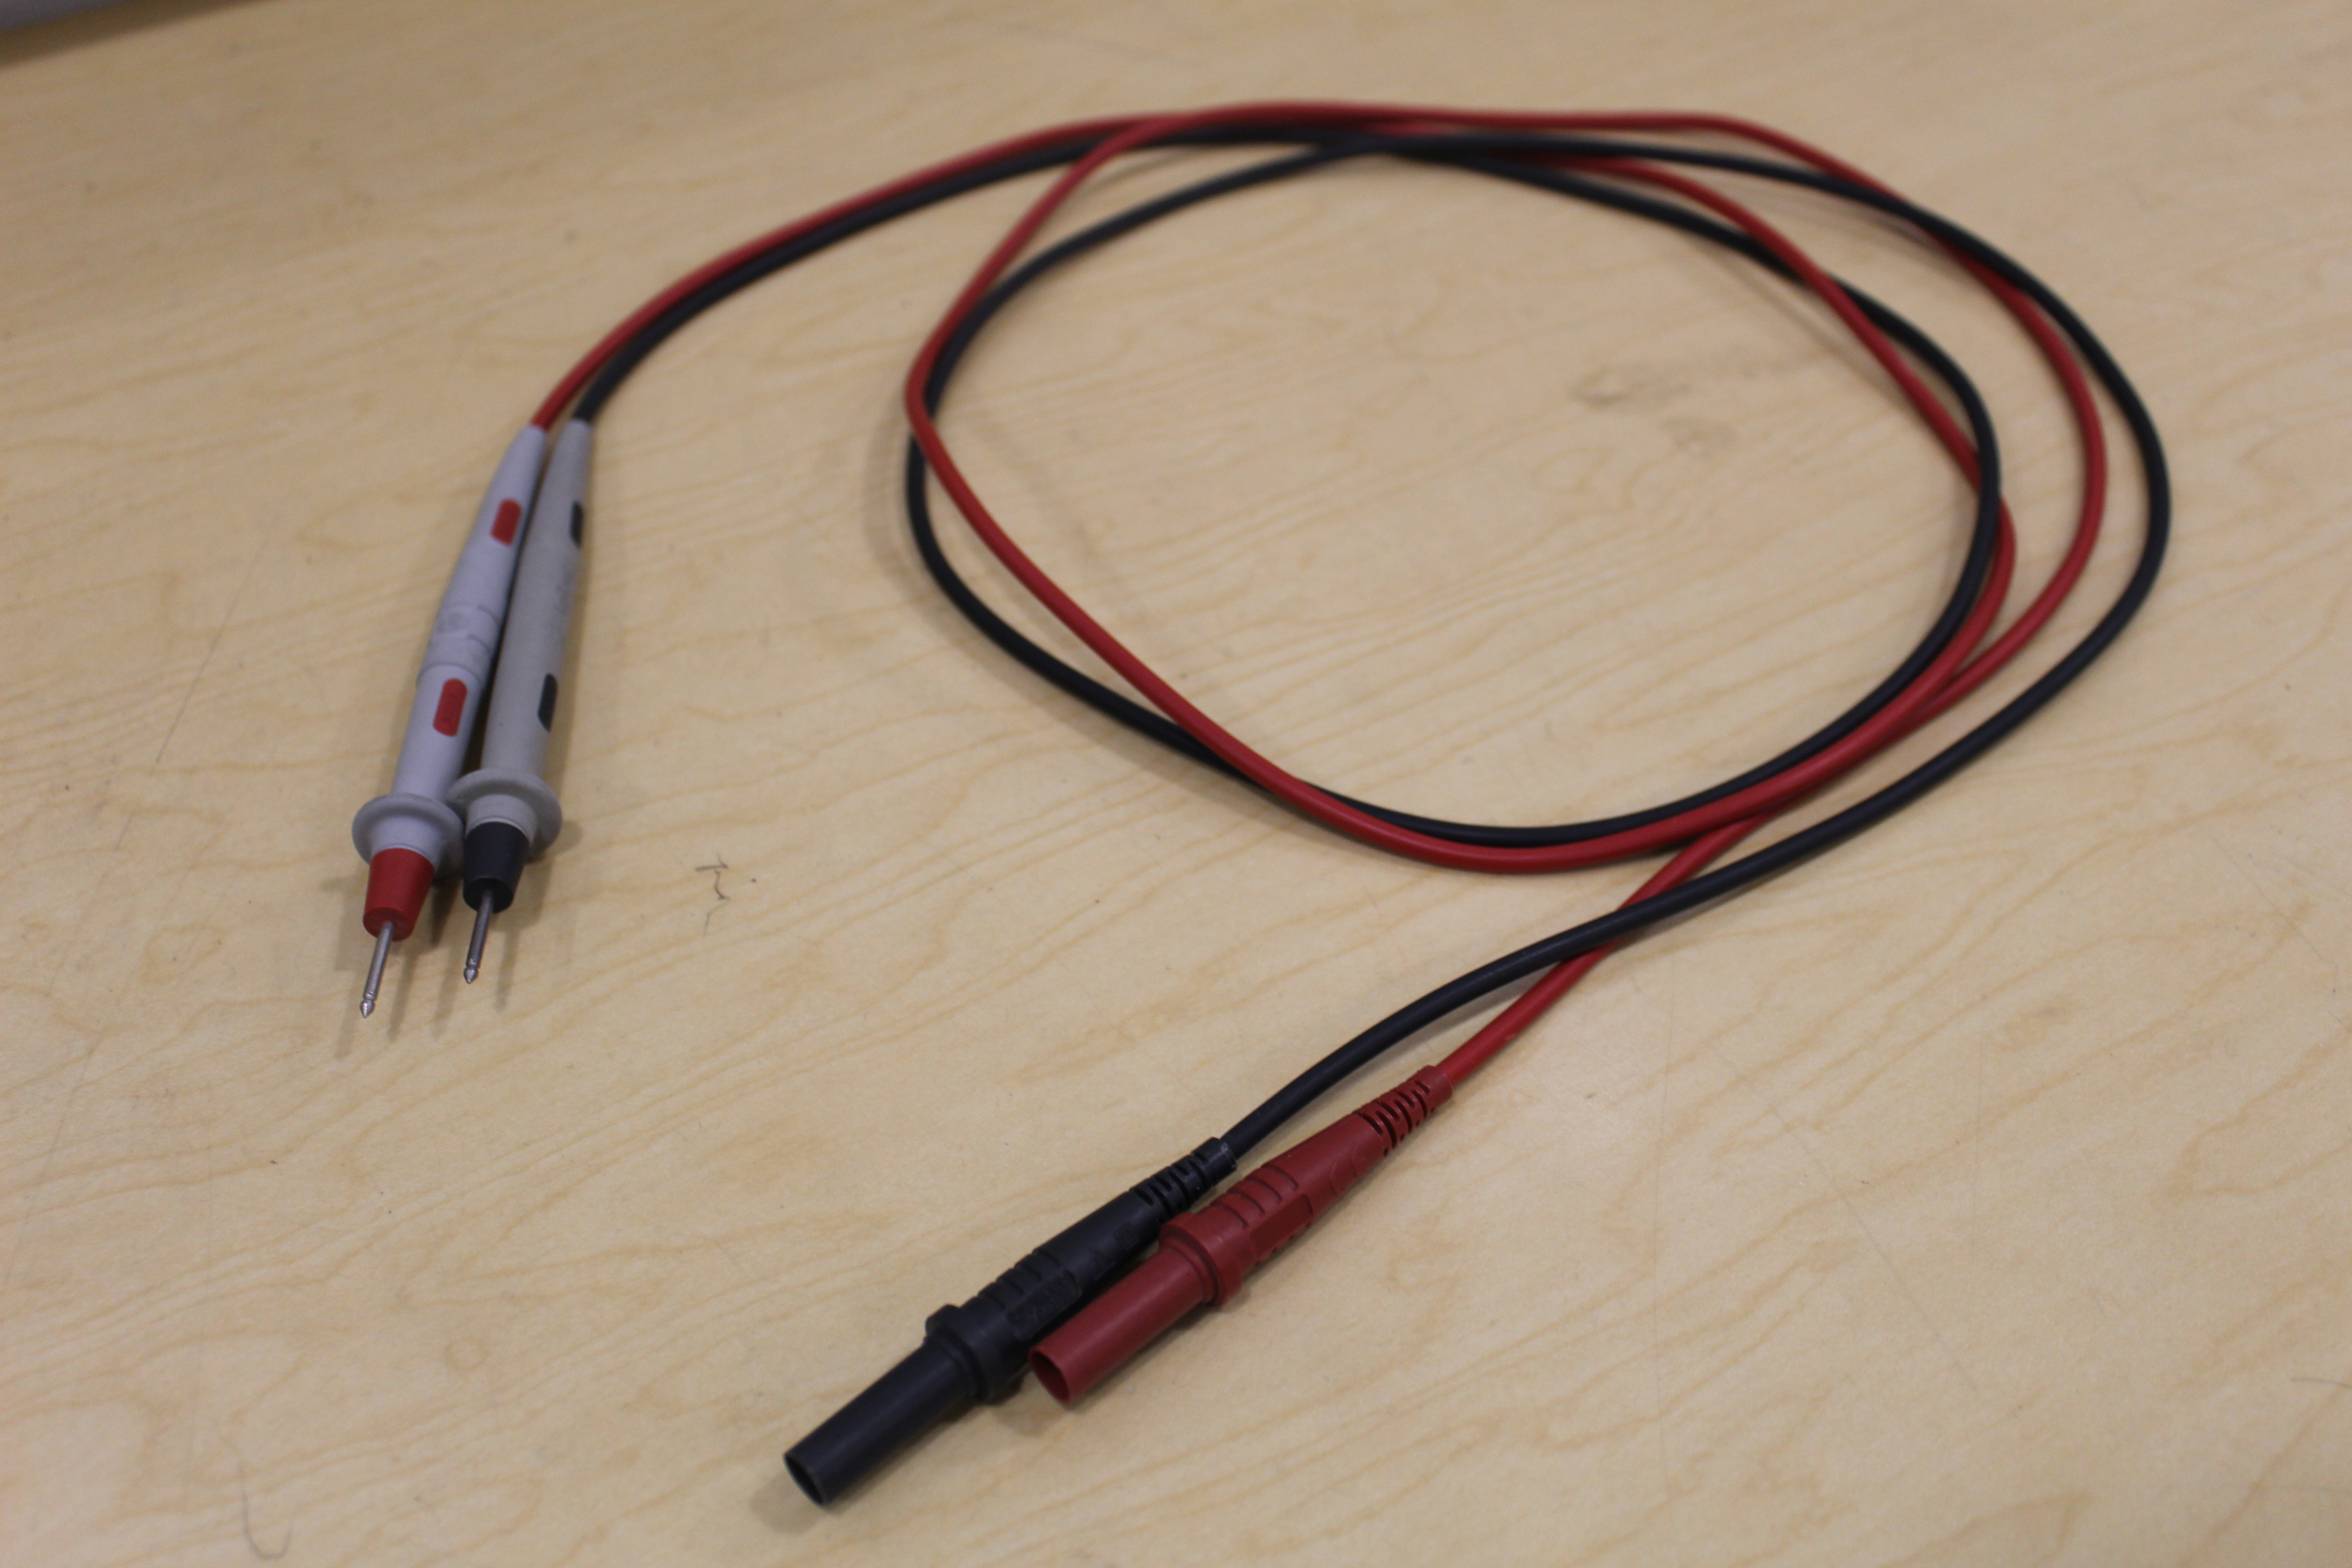
\includegraphics[width=1\linewidth]{photos/prelim/dmmcable.JPG}
  \caption{DMM cables with probe tips.}
\end{subfigure}
\caption{Examples of a DMM and its cables.}
\end{figure}

The DMM uses the cables to probe a circuit at some points and measure values such as current, voltage, and resistance at any by selecting the appropriate measurement setting and interface terminal on the devices front panel. To measure some value, the circular end of the black and red probe cables in \textit{Figure 14(b)} are attached to the appropriate ports on the DMM. The pointy probe side of the two cables are then used to interact with the circuit at the desired location. When the measurement is completed, the desired value is displayed on the multimeters screen. Measuring resistance is as simple as placing the black probes tip on one wire of the resistor and red probes tip on the other wire, putting the red DMM cable in the port with the $\Omega$ and black cable in the LO port, and selecting the $\Omega$ button on the front panel of the DMM. The value of resistance will then be displayed on the screen of the DMM.

To measure voltage, the probing is as simple as placing the tips of the red and black leads across which the potential difference is to be measured in an active circuit. For example, consider the circuit schematic in \textit{Figure 14(a)}. To measure the voltage drop across the resistor R, the red lead is placed at the wire connecting $V_1$ and the black lead at $V_2$. If $V_1 = 5V$ and $V_2 = 2V$, then the DMM would read a voltage of 3V. If the black lead is moved to the ground wire at the bottom of the circuit, then the DMM would then read the voltage of $V_1$, which would be 5V.

To measure current, the DMM must have the current of the circuit flow through the leads and back into the circuit. For this reason, the circuit must be "broken" in the sense that the location where current is to be measured must go into the red lead and out of the black lead in the same place. For example, in the circuit in \textit{Figure 15(b)} if the current flowing through the resistor is to be measured, the DMM must break the wire as shown. If $V_1 = 5V$, $V_2 = 2V$, and $R = 3k\Omega$, then the DMM would read a current value of 1 mA. The current is the same if taken to the left or right of the resistor.

\begin{figure}[H]
\begin{subfigure}{.5\textwidth}
  \centering
  \includegraphics[width=0.6\linewidth]{photos/prelim/circuitschmeatic_voltage.PNG}
  \caption{Measuring the voltage across the resistor.}
\end{subfigure}%
\begin{subfigure}{.5\textwidth}
  \centering
  \includegraphics[width=0.6\linewidth]{photos/prelim/circuitschmeatic_current.PNG}
  \caption{Measuring the current through the resistor.}
\end{subfigure}
\caption{Examples of how to measure voltage and current in the circuit with a DMM.}
\end{figure}

\subsection{Oscilloscopes}

\begin{figure}[H]
    \centering
    \includegraphics[width=15cm]{photos/prelim/oscilloscope.jpg}
    \caption{A 2-channel digital storage oscilloscope.}
\end{figure}

Oscilloscopes are useful for plotting the variations of the voltages over time, as occurs in AC voltages. Although they are most useful for AC waveforms, oscilloscopes can also measure DC signals. In contrast to DMMs, oscilloscopes can plot the voltage that is being input to the oscilloscope against time instead of providing the user with an instantaneous voltage reading. In this respect, the oscilloscope takes several voltage measurements over time, stores them into memory, and then plots them on a grid on the screen for observation, as seen in \textit{Figure 16}. 

Notice on the screen the $100mV/$ and $200\mu s/$ at the top of the screen. These refer to the scaling of the displays waveform on the grid in terms of the x (time) axis and y (voltage) axis. These scaling values refer to how much each division or line in the grid of the graph in each axis direction represents. To calculate the amount of voltage present at any point in time on the display, you would calculate the number of divisions of displacement from the ground indicator by the scaling value. For example, in the waveform seen in \textit{Figure 16}, the highest peak goes about 2 divisions above the center and the lowest peak goes about 2 divisions below. Since the reference voltage is in the center of the grid, as dictated by the indicator on the far left side of the screen, the highest peak occurs at $+2 divs * 100\frac{mV}{divs} = +200mV$ and the lowest at $-2 divs * 100\frac{mV}{divs} = -200mV$. This means the wave for has a $V_p = 200mV$ and $V_{pp} = 200 - (-200) mV = 400 mV$

This display of the waveform is useful for diagnosis of circuit behavior by understanding what is happening both qualitatively and quantitatively. As well as being able to display the waveforms voltage against time, oscilloscope typically have additional mathematical operation features such as computing parameters such as peak voltages and frequency and the Fast Fourier Transform. These features enable an electrical engineer to quickly analyze a circuit and help make an oscilloscope a fundamental tool in the lab.

\end{document}